\section{Analysis of Standard Strategies}
\label{sec:eval-common-strategies}

We first 
we evaluated standard tiebreaking strategies for domain-independent cost-optimal
classical planning and analyze their performance differences.  
In our experiments, all planners are based on Fast
Downward, and all experiments are run with a 5-minute,
4GB memory limit for the search binary (FD translation/preprocessing
times are not included in the 5-minute limit).  All experiments were
conducted on Xeon E5410@2.33GHz CPUs. For the randomized configurations, we took the average of 10 runs.
% 
We used two \sota heuristic functions \lmcut \cite{Helmert2009} and \mands \cite{HelmertHHN14} as the primary
heuristic functions used for calculating $f$ and $h$.  For \mands, we used the currently recommended
settings\footnote{http://www.fast-downward.org/Doc/Heuristic\#Merge-and-shrink\_heuristic as of \today}
(bisimulation-based shrink strategy, DFP merge strategy and exact label reduction).  These basic experimental
configurations are shared in all performance evaluation experiments throughout this paper. 

% following paragraph is added in order to avoid repeating the list of domains not
% included due to no coverage difference.
We used 1104 instances from 35 standard benchmark domains. These
instances are those originally included in the test suite included with the Fast
Downward planning system. In detail, they are: \pddl{airport}(50),
\pddl{barman-opt11}(20), \pddl{blocks}(35), \pddl{cybersec}(19), \pddl{depot}(22), \pddl{driverlog}(20),
\pddl{elevators-opt11}(20), \pddl{floortile-opt11}(20), \pddl{freecell}(80), \pddl{grid}(5),
\pddl{gripper}(20), \pddl{hanoi}(30), \pddl{logistics00}(28), \pddl{miconic}(150), \pddl{mprime}(35),
\pddl{mystery}(30), \pddl{nomystery-opt11}(20), \pddl{openstacks-opt11}(20),
\pddl{parcprinter-opt11}(20), \pddl{parking-opt11}(20), \pddl{pathways}(30),
\pddl{pegsol-opt11}(20), \pddl{pipesworld-notankage}(50), \pddl{pipesworld-tankage}(50),
\pddl{psr-small}(50), \pddl{rovers}(40), \pddl{scanalyzer-opt11}(20), \pddl{sokoban-opt11}(20),
\pddl{storage}(30), \pddl{tidybot-opt11}(20), \pddl{tpp}(30), \pddl{transport-opt11}(20),
\pddl{visitall-opt11}(20), \pddl{woodworking-opt11}(20), \pddl{zenotravel}(20).

\subsection{Is $h$-Based Tiebreaking Necessary?}

\label{sec:noh}
\todo*{changed order because the next 2 sections discuss the importance of default tiebreaking, which is directly caused by the size of plateaus, so they should be consecutive; this section is not directly related and seemed out of place sandwiched between defaults and plateaus}
As noted above in Section \ref{sec:astar-background}, the current standard practice is to use a tiebreaking criterion which uses the $h$-value of the nodes. However, to our knowledge, the need for $h$-based tiebreaking has not been previously empirically investigated.

In \reftbl{tbl:summary-std}, we show the summary results for $[f, \fifo]$ and $[f, \lifo]$, the
\astar variants which rely on \fifo or \lifo default tiebreaking only, as well as the standard $[f, h, \fifo]$ and $[f, h, \lifo]$ strategies.
(detailed results are in
\reftbl{tbl:lmcut-ipc-std} and \reftbl{tbl:mands-ipc-std}.
$[f,\lifo]$, which simply breaks ties among nodes with the same
$f$-cost by expanding the most recently generated nodes first
\cite{korf1985depth}, clearly dominates $[f,\fifo]$.  Interestingly,
the performance of the $[f,\lifo]$ strategy is comparable to
$[f,h,\lifo]$ and $[f,h,\fifo]$.  This may be surprising, considering
the ubiquity of $h$-based tiebreaking in the search and planning
communities.

This is explained by the fact that 
\lifo behaves somewhat similarly to $h$-based tiebreaking.
\lifo expands the most recently generated node $n$.
For any child $n'$, 
if the heuristic function is admissible and $f(n') = f(n)$, there are only 2 possibilities :
(1) $g(n') > g(n)$ and $h(n') < h(n)$, or
(2) $g(n') = g(n)$ and $h(n') = h(n)$,
because $g(n)+h(n)=g(n')+h(n')$.
Thus, as \lifo expands nodes in a ``depth-first'' manner,
the nodes that continue to be expanded in the plateau by \lifo usually   %added ``usually' because usually true, but not always true because LIFO/DFS has to periodically ``back up'' to nodes with h > h(n)  after exhausiting  nodes with h=h(n).
have non-increasing $h$-values,
much like in $h$-based tiebreaking which always searches toward the least $h$ cost.
Thus, although the expansion order of $[f,\lifo]$ is not exactly the same as that of $h$-based tiebreaking strategies,
their performance is similar.

% \textbf{An in-depth investigation of the behavior of $[f,\lifo]$ vs. $h$-based tiebreaking is a direction for future work.}
% Compared to the $h$-based variants which explicitly selects nodes with smaller $h$ and its expanded nodes have non-increasing $h$-values,
% This has the same  can behave somewhat similarly to actively expanding nodes with low $h$-values, as done by $h$-based tiebreaking.
% \citeauthor{burns2012implementing}
% (\citeyear{burns2012implementing}) writes ``the goal can be found more
% quickly in the final $f$ layer of search'' about $h$ tiebreaking.


\subsection{Do Default Strategies Make a Difference?}

Next, we  compared two commonly used tiebreaking strategies, $[f,h,\fifo]$, $[f,h,\lifo]$, which
first break ties according to $h$, and then apply \fifo or \lifo
default tiebreaking, respectively.
Summary results for \lmcut and \mands are
shown in \reftbl{tbl:summary-std}, and the detailed results are in \reftbl{tbl:lmcut-ipc-std} and \reftbl{tbl:mands-ipc-std}.
Differences in coverage are observed in several domains and $[f,h,\lifo]$ outperforms $[f,h,\fifo]$ overall. Thus, the choice of default criterion seems to have a modest but measurable impact when the first tiebreaking criterion is $h$.

We also conducted experiments using \ro (Random Order) default tiebreaking because it is another trivial way to
break ties. We ran the experiments 10 times with the different random seeds, then took the average and the
standard deviation of the coverages. The performance of \ro is comparable to \fifo default tiebreaking regardless
of the primary heuristics, or the presence of $h$-based tiebreaking.
\todo*{The baseline [f,h,ro] and [f,ro] are in the tables, but don't seem to be defined/mentioned/discussed at all in this section}

\begin{table}[htbp]
 {
 \centering
 \begin{center}
\begin{tabular}{|l|cc|}
Sorting Criteria & IPC(1104) & IPC(1104)\\
 & \lmcut & \mands\\
 &  & \\
\([f,\fifo]\) & 443 & 460\\
\([f,\lifo]\) & 558 & 490\\
\([f,\ro]\) & 448.9 \(\pm\) 1.3 & 460.9 \(\pm\) 1.6\\
\([f,h,\fifo]\) & 558 & 491\\
\([f,h,\lifo]\) & \textbf{565} & \textbf{496}\\
\([f,h,\ro]\) & 558.9 \(\pm\) 2.1 & 489.4 \(\pm\) 1.0\\
\end{tabular}
\end{center}

 \caption{
 Summary of coverage comparison (the number of instances solved in 5min, 4GB, LMcut
 heuristics) among
 the standard baseline tiebreaking algorithms (details in \reftbl{tbl:lmcut-ipc-std} and \reftbl{tbl:mands-ipc-std}, leftmost 2 columns). 
 }
 \label{tbl:summary-std}
 }
\end{table}


\begin{table}[htbp]
 {
 \centering
 \begin{center}
\begin{tabular}{|r|*{2}{ccc|}}
Domain & \([f,\fifo]\) & \([f,\lifo]\) & \([f,\ro]\) & \([f,h,\fifo]\) & \([f,h,\lifo]\) & \([f,h,\ro]\)\\
IPC benchmark (1104) & 443 & 558 & 448.9 \(\pm\) 1.3 & 558 & \textbf{565} & 558.9 \(\pm\) 2.1\\
airport(50) & 18 & 26 & 18 \(\pm\) 0 & \textbf{27} & 26 & 25.7 \(\pm\) 0.5\\
barman-opt11(20) & 0 & 0 & 0 \(\pm\) 0 & 0 & 0 & 0 \(\pm\) 0\\
blocks(35) & 26 & 26 & 26 \(\pm\) 0 & \textbf{28} & \textbf{28} & \textbf{28} \(\pm\) 0\\
\textbf{cybersec(19)} & 0 & 3 & 0 \(\pm\) 0 & 2 & 3 & \textbf{3.9} \(\pm\) 1.1\\
depot(22) & 5 & 5 & 5 \(\pm\) 0 & 6 & 6 & 6 \(\pm\) 0\\
driverlog(20) & 12 & 13 & 12 \(\pm\) 0 & 13 & 13 & 13 \(\pm\) 0\\
elevators-opt11(20) & 14 & 15 & 14 \(\pm\) 0 & 15 & 15 & 15 \(\pm\) 0\\
floortile-opt11(20) & 6 & 6 & 6 \(\pm\) 0 & 6 & 6 & 6 \(\pm\) 0\\
freecell(80) & 8 & 9 & 8.7 \(\pm\) 0.5 & 9 & 9 & 9 \(\pm\) 0\\
grid(5) & 1 & 1 & 1 \(\pm\) 0 & 1 & 1 & 1 \(\pm\) 0\\
gripper(20) & 6 & 6 & 6 \(\pm\) 0 & 6 & 6 & 6 \(\pm\) 0\\
hanoi(30) & 12 & 12 & 12 \(\pm\) 0 & 12 & 12 & 12 \(\pm\) 0\\
logistics00(28) & 16 & 18 & 16 \(\pm\) 0 & \textbf{20} & \textbf{20} & \textbf{20} \(\pm\) 0\\
miconic(150) & 68 & 140 & 68 \(\pm\) 0 & 140 & 140 & 140 \(\pm\) 0\\
mprime(35) & 20 & \textbf{22} & 19.9 \(\pm\) 0.3 & 21 & 21 & 20.9 \(\pm\) 0.3\\
mystery(30) & 15 & 16 & 15 \(\pm\) 0 & 16 & 16 & 15.2 \(\pm\) 0.4\\
nomystery-opt11(20) & 12 & 13 & 12 \(\pm\) 0 & \textbf{14} & \textbf{14} & \textbf{14} \(\pm\) 0\\
\textbf{openstacks-opt11(20)} & 11 & \textbf{18} & 11.2 \(\pm\) 0.4 & 11 & \textbf{18} & 11.7 \(\pm\) 0.5\\
parcprinter-opt11(20) & 12 & 13 & 12 \(\pm\) 0 & 13 & 13 & 13 \(\pm\) 0\\
parking-opt11(20) & 1 & 1 & 1 \(\pm\) 0 & 1 & 1 & 1 \(\pm\) 0\\
pathways(30) & 4 & 5 & 4 \(\pm\) 0 & 5 & 5 & 5 \(\pm\) 0\\
pegsol-opt11(20) & 17 & 17 & 17 \(\pm\) 0 & 17 & 17 & 17 \(\pm\) 0\\
pipesworld-notankage(50) & 13 & 13 & 13 \(\pm\) 0 & 14 & 14 & 14.6 \(\pm\) 0.5\\
pipesworld-tankage(50) & 7 & 8 & 8 \(\pm\) 0 & 8 & 8 & 8 \(\pm\) 0\\
psr-small(50) & 48 & 48 & 48 \(\pm\) 0 & 48 & 48 & 48 \(\pm\) 0\\
rovers(40) & 7 & 7 & 7 \(\pm\) 0 & 7 & 7 & 7 \(\pm\) 0\\
scanalyzer-opt11(20) & 4 & \textbf{10} & 5.4 \(\pm\) 0.7 & \textbf{10} & \textbf{10} & \textbf{10} \(\pm\) 0\\
sokoban-opt11(20) & 19 & 19 & 19 \(\pm\) 0 & 19 & 19 & 19 \(\pm\) 0\\
storage(30) & 14 & 14 & 14 \(\pm\) 0 & 14 & 14 & 14 \(\pm\) 0\\
tidybot-opt11(20) & 11 & 12 & 11 \(\pm\) 0 & 12 & 12 & 12 \(\pm\) 0\\
tpp(30) & 6 & 6 & 6 \(\pm\) 0 & 6 & 6 & 6 \(\pm\) 0\\
transport-opt11(20) & 6 & 6 & 6 \(\pm\) 0 & 6 & 6 & 6 \(\pm\) 0\\
visitall-opt11(20) & 9 & 10 & 9.4 \(\pm\) 0.5 & 10 & 10 & 10 \(\pm\) 0\\
woodworking-opt11(20) & 6 & 9 & 8.2 \(\pm\) 0.4 & \textbf{10} & \textbf{10} & \textbf{10} \(\pm\) 0\\
zenotravel(20) & 9 & \textbf{11} & 9 \(\pm\) 0 & \textbf{11} & \textbf{11} & \textbf{11} \(\pm\) 0\\
\end{tabular}
\end{center}

 \caption{
 Coverage comparison (the number of instances solved in 5min, 4GB, LMcut
 heuristics) among
 the standard baseline tiebreaking algorithms. We highlight the
 best results when the difference between the maximum and the minimum coverage exceeds 2.
 }
 \label{tbl:lmcut-ipc-std}
 }
\end{table}

\begin{table}[htbp]
 {
 \centering
 \begin{center}
\begin{tabular}{|r|*{2}{ccc|}}
Domain & $[f,\fifo]$ & $[f,\lifo]$ & $[f,\ro]$ & $[f,h,\fifo]$ & $[f,h,\lifo]$ & $[f,h,\ro]$\\
IPC benchmark (1104) & 460 & 490 & 460.9 $\pm$ 1.6 & 491 & \textbf{496} & 489.4 $\pm$ 1.0\\
airport(50) & 9 & 9 & 9 $\pm$ 0 & 9 & 9 & 9 $\pm$ 0\\
barman-opt11(20) & 4 & 4 & 4 $\pm$ 0 & 4 & 4 & 4 $\pm$ 0\\
blocks(35) & 21 & 22 & 21 $\pm$ 0 & 22 & 22 & 22 $\pm$ 0\\
\textbf{cybersec(19)} & 0 & 0 & 0 $\pm$ 0 & 0 & 0 & 0 $\pm$ 0\\
depot(22) & 5 & 6 & 5 $\pm$ 0 & 6 & 6 & 5 $\pm$ 0\\
driverlog(20) & 12 & 12 & 12 $\pm$ 0 & 12 & 12 & 12 $\pm$ 0\\
elevators-opt11(20) & 13 & 13 & 13 $\pm$ 0 & 13 & 13 & 13 $\pm$ 0\\
floortile-opt11(20) & 5 & 6 & 5 $\pm$ 0 & 6 & 6 & 6 $\pm$ 0\\
freecell(80) & 15 & 16 & 15 $\pm$ 0 & \textbf{17} & \textbf{17} & 16 $\pm$ 0\\
grid(5) & 2 & 2 & 2 $\pm$ 0 & 2 & 2 & 2 $\pm$ 0\\
gripper(20) & 8 & \textbf{20} & 8 $\pm$ 0 & \textbf{20} & \textbf{20} & \textbf{20} $\pm$ 0\\
hanoi(30) & 14 & 14 & 14 $\pm$ 0 & 14 & 14 & 14 $\pm$ 0\\
logistics00(28) & 20 & 20 & 20 $\pm$ 0 & 20 & 20 & 20 $\pm$ 0\\
miconic(150) & 68 & \textbf{73} & 68.3 $\pm$ 0.7 & \textbf{73} & \textbf{73} & \textbf{73.2} $\pm$ 0.4\\
mprime(35) & 23 & 23 & 22 $\pm$ 0 & 23 & \textbf{24} & 23.7 $\pm$ 0.5\\
mystery(30) & 15 & 15 & 15 $\pm$ 0 & 15 & 16 & 15 $\pm$ 0\\
nomystery-opt11(20) & 17 & 18 & 17.8 $\pm$ 0.4 & 18 & 18 & 18 $\pm$ 0\\
\textbf{openstacks-opt11(20)} & 15 & \textbf{19} & 15.4 $\pm$ 0.5 & 15 & \textbf{19} & 15.4 $\pm$ 0.5\\
parcprinter-opt11(20) & 10 & 10 & 10 $\pm$ 0 & 10 & 10 & 10 $\pm$ 0\\
parking-opt11(20) & 1 & 1 & 1 $\pm$ 0 & 1 & 1 & 1 $\pm$ 0\\
pathways(30) & 4 & 4 & 4 $\pm$ 0 & 4 & 4 & 4 $\pm$ 0\\
pegsol-opt11(20) & 17 & \textbf{19} & 17.2 $\pm$ 0.4 & \textbf{19} & \textbf{19} & \textbf{19} $\pm$ 0\\
pipesworld-notankage(50) & 9 & 9 & 8.9 $\pm$ 0.3 & 10 & 10 & 9.9 $\pm$ 0.3\\
pipesworld-tankage(50) & 13 & 13 & 13.1 $\pm$ 0.3 & 13 & 13 & 13.2 $\pm$ 0.4\\
psr-small(50) & 50 & 50 & 50 $\pm$ 0 & 50 & 50 & 50 $\pm$ 0\\
rovers(40) & 6 & \textbf{8} & 6.1 $\pm$ 0.3 & \textbf{8} & \textbf{8} & \textbf{8} $\pm$ 0\\
scanalyzer-opt11(20) & 10 & 10 & 10 $\pm$ 0 & 10 & 10 & 10 $\pm$ 0\\
sokoban-opt11(20) & 20 & 20 & 20 $\pm$ 0 & 20 & 20 & 20 $\pm$ 0\\
storage(30) & 15 & 15 & 15 $\pm$ 0 & 15 & 15 & 15 $\pm$ 0\\
tidybot-opt11(20) & 0 & 0 & 0 $\pm$ 0 & 0 & 0 & 0 $\pm$ 0\\
tpp(30) & 6 & 6 & 6 $\pm$ 0 & 7 & 6 & 6 $\pm$ 0\\
transport-opt11(20) & 7 & 7 & 7 $\pm$ 0 & 7 & 7 & 7 $\pm$ 0\\
visitall-opt11(20) & 9 & 9 & 9 $\pm$ 0 & 9 & 9 & 9 $\pm$ 0\\
woodworking-opt11(20) & 7 & 7 & 7 $\pm$ 0 & 7 & 7 & 7 $\pm$ 0\\
zenotravel(20) & 10 & 10 & 10 $\pm$ 0 & \textbf{12} & \textbf{12} & \textbf{12} $\pm$ 0\\
\end{tabular}
\end{center}

 \caption{
 Coverage comparison (the number of instances solved in 5min, 4GB, M\&S heuristics) among
 the standard baseline tiebreaking algorithms. We highlight the
 best results when the difference between the maximum and the minimum coverage exceeds 2.
 }
 \label{tbl:mands-ipc-std}
 }
\end{table}


\subsection{Plateaus and Tiebreaking}

\refig{fig:f-h-eval} provides a
more fine-grained analysis by comparing the number of node evaluations
(calls to the expensive \lmcut heuristic function) in each instance between $[f,h,\lifo]$ and $[f,h,\fifo]$ strategies.
The difference in the number of nodes
evaluated can sometimes be larger than a factor of 10 (\pddl{Openstacks}, \pddl{Cybersec} domains).
As noted in Section \ref{sec:astar-background}, the choice among default criteria has not been considered very important in the literature, as evidenced by the lack of explicit descriptions of the default tiebreaking criterion in recent papers. 
Our results suggest that 2nd-level default tiebreaking can have a surprisingly large effect on
the search performance.

\begin{figure}[htbp]
 \centering \relsize{-3}
 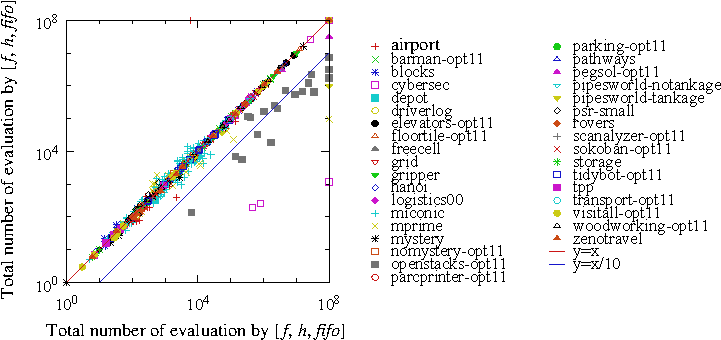
\includegraphics[width=\linewidth]{tables/aaai16-30min-5min-cut/aaai16prelim3/evaluated-lmcut_ff-lmcut_lf.pdf}
 \caption{The number of LMcut evaluations on various IPC planning benchmark domains,
 with standard \fifo vs \lifo default tiebreaking, both with $h$
 tiebreaking. \lifo evaluates  less than $1/10$ of the nodes evaluated
 by \fifo in \pddl{Cybersec} and \pddl{Openstacks}. 
 }
 \label{fig:f-h-eval}
\end{figure}

The effect of the choice of 2nd-level default tiebreaking criteria (\lifo vs.
\fifo)  when the 1st-level tiebreaking criterion is  $h$-tiebreaking is
limited to each search plateau $\plateau{f,h}$, the set of nodes which
share the same $f$ value and $h$ value.
% 
Also, in admissible search, two \astar implementations using 
different default tiebreaking criteria both expand the same set of
nodes in the region where $f<f^*$.
% 
Furthermore, nodes with $h>0$ can not be goal nodes when $h$ is admissible.
% 
Therefore, the effect of default tiebreaking becomes most prominent in the final plateau, $\plateau{f^*,0}$.

% Conventionally, 
% this final plateau, $\plateau{f^*,0}$, was naively considered to be very small compared to the
% total size of the search space required to be expanded by \astar.
% However, 
Counterintuitively, the $\plateau{f^*, 0}$ region can be large enough to
cause a significant performance difference -- in fact, this final plateau can even account for \emph{most} of the
search effort required by \astar.
\refig{fig:plateau} plots the size of the final plateau on 1104 IPC
benchmark instances.  The $y$-axis represents the number of nodes within
the final plateau ($f=f^*, h=0$), and the $x$-axis represents the total
number of nodes expanded so far. This figure suggests that in some
domains such as \pddl{Openstacks} and \pddl{Cybersec}, the planner
spends most of the runtime searching the final plateau for a solution,
even with the help of $h$ tiebreaking.
\todo{maybe we need a statistics on (\#goal)/(\#states) ?}

A natural question is:  What makes these two domains
(\pddl{Openstacks} and \pddl{Cybersec})  different from all other domains
which have much smaller final plateaus?

\begin{figure}[htbp]
   \centering
  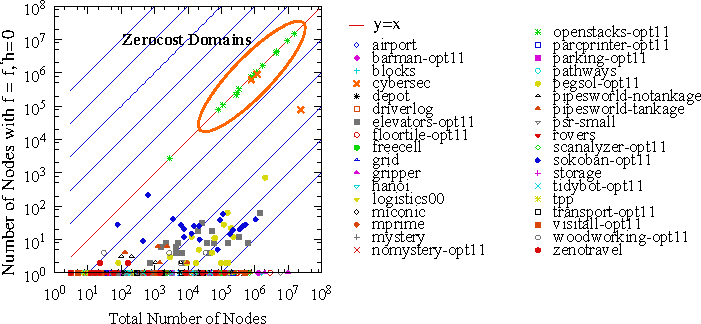
\includegraphics[width=\linewidth]{tables/aaai16-frontier/aaai16prelim3/lmcut_frontier-front.pdf}
  \caption{
 The number of nodes with $f=f^*, h=0$ (y-axis), which form
  the final plateau when 1st-level tiebreaking is according to $h$, compared to
  the total number of nodes in the search space (x-axis) with $f\leq
  f^*$ on 1104 IPC benchmark problems.  Note that \pddl{Openstacks}
  and \pddl{Cybersec} instances are near the $y=x$ line.
  These statistics are obtained by running a modified Fast Downward with
 \lmcut which continues searching after the solution is found
 until all nodes with cost $f=f^*$ are expanded.} \label{fig:plateau}
\end{figure}

